\documentclass[1p]{elsarticle_modified}
%\bibliographystyle{elsarticle-num}

%\usepackage[colorlinks]{hyperref}
%\usepackage{abbrmath_seonhwa} %\Abb, \Ascr, \Acal ,\Abf, \Afrak
\usepackage{amsfonts}
\usepackage{amssymb}
\usepackage{amsmath}
\usepackage{amsthm}
\usepackage{scalefnt}
\usepackage{amsbsy}
\usepackage{kotex}
\usepackage{caption}
\usepackage{subfig}
\usepackage{color}
\usepackage{graphicx}
\usepackage{xcolor} %% white, black, red, green, blue, cyan, magenta, yellow
\usepackage{float}
\usepackage{setspace}
\usepackage{hyperref}

\usepackage{tikz}
\usetikzlibrary{arrows}

\usepackage{multirow}
\usepackage{array} % fixed length table
\usepackage{hhline}

%%%%%%%%%%%%%%%%%%%%%
\makeatletter
\renewcommand*\env@matrix[1][\arraystretch]{%
	\edef\arraystretch{#1}%
	\hskip -\arraycolsep
	\let\@ifnextchar\new@ifnextchar
	\array{*\c@MaxMatrixCols c}}
\makeatother %https://tex.stackexchange.com/questions/14071/how-can-i-increase-the-line-spacing-in-a-matrix
%%%%%%%%%%%%%%%

\usepackage[normalem]{ulem}

\newcommand{\msout}[1]{\ifmmode\text{\sout{\ensuremath{#1}}}\else\sout{#1}\fi}
%SOURCE: \msout is \stkout macro in https://tex.stackexchange.com/questions/20609/strikeout-in-math-mode

\newcommand{\cancel}[1]{
	\ifmmode
	{\color{red}\msout{#1}}
	\else
	{\color{red}\sout{#1}}
	\fi
}

\newcommand{\add}[1]{
	{\color{blue}\uwave{#1}}
}

\newcommand{\replace}[2]{
	\ifmmode
	{\color{red}\msout{#1}}{\color{blue}\uwave{#2}}
	\else
	{\color{red}\sout{#1}}{\color{blue}\uwave{#2}}
	\fi
}

\newcommand{\Sol}{\mathcal{S}} %segment
\newcommand{\D}{D} %diagram
\newcommand{\A}{\mathcal{A}} %arc


%%%%%%%%%%%%%%%%%%%%%%%%%%%%%5 test

\def\sl{\operatorname{\textup{SL}}(2,\Cbb)}
\def\psl{\operatorname{\textup{PSL}}(2,\Cbb)}
\def\quan{\mkern 1mu \triangleright \mkern 1mu}

\theoremstyle{definition}
\newtheorem{thm}{Theorem}[section]
\newtheorem{prop}[thm]{Proposition}
\newtheorem{lem}[thm]{Lemma}
\newtheorem{ques}[thm]{Question}
\newtheorem{cor}[thm]{Corollary}
\newtheorem{defn}[thm]{Definition}
\newtheorem{exam}[thm]{Example}
\newtheorem{rmk}[thm]{Remark}
\newtheorem{alg}[thm]{Algorithm}

\newcommand{\I}{\sqrt{-1}}
\begin{document}

%\begin{frontmatter}
%
%\title{Boundary parabolic representations of knots up to 8 crossings}
%
%%% Group authors per affiliation:
%\author{Yunhi Cho} 
%\address{Department of Mathematics, University of Seoul, Seoul, Korea}
%\ead{yhcho@uos.ac.kr}
%
%
%\author{Seonhwa Kim} %\fnref{s_kim}}
%\address{Center for Geometry and Physics, Institute for Basic Science, Pohang, 37673, Korea}
%\ead{ryeona17@ibs.re.kr}
%
%\author{Hyuk Kim}
%\address{Department of Mathematical Sciences, Seoul National University, Seoul 08826, Korea}
%\ead{hyukkim@snu.ac.kr}
%
%\author{Seokbeom Yoon}
%\address{Department of Mathematical Sciences, Seoul National University, Seoul, 08826,  Korea}
%\ead{sbyoon15@snu.ac.kr}
%
%\begin{abstract}
%We find all boundary parabolic representation of knots up to 8 crossings.
%
%\end{abstract}
%\begin{keyword}
%    \MSC[2010] 57M25 
%\end{keyword}
%
%\end{frontmatter}

%\linenumbers
%\tableofcontents
%
\newcommand\colored[1]{\textcolor{white}{\rule[-0.35ex]{0.8em}{1.4ex}}\kern-0.8em\color{red} #1}%
%\newcommand\colored[1]{\textcolor{white}{ #1}\kern-2.17ex	\textcolor{white}{ #1}\kern-1.81ex	\textcolor{white}{ #1}\kern-2.15ex\color{red}#1	}

{\Large $\underline{12n_{0126}~(K12n_{0126})}$}

\setlength{\tabcolsep}{10pt}
\renewcommand{\arraystretch}{1.6}
\vspace{1cm}\begin{tabular}{m{100pt}>{\centering\arraybackslash}m{274pt}}
\multirow{5}{120pt}{
	\centering
	\includegraphics[width=112pt]{../../../GIT/diagram.site/Diagrams/png/2215_12n_0126.png}\\
\ \ \ A knot diagram\footnotemark}&
\allowdisplaybreaks
\textbf{Linearized knot diagam} \\
\cline{2-2}
 &
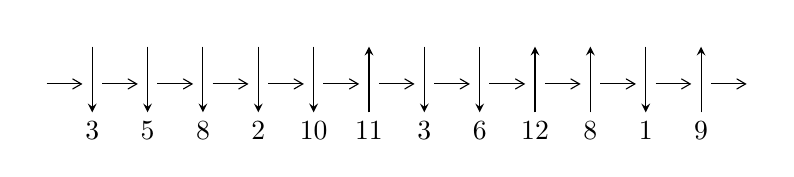
\begin{tikzpicture}[x=20pt, y=17pt]
	% nodes
	\node (C0) at (0, 0) {};
	\node (C1) at (1, 0) {};
	\node (C1U) at (1, +1) {};
	\node (C1D) at (1, -1) {3};

	\node (C2) at (2, 0) {};
	\node (C2U) at (2, +1) {};
	\node (C2D) at (2, -1) {5};

	\node (C3) at (3, 0) {};
	\node (C3U) at (3, +1) {};
	\node (C3D) at (3, -1) {8};

	\node (C4) at (4, 0) {};
	\node (C4U) at (4, +1) {};
	\node (C4D) at (4, -1) {2};

	\node (C5) at (5, 0) {};
	\node (C5U) at (5, +1) {};
	\node (C5D) at (5, -1) {10};

	\node (C6) at (6, 0) {};
	\node (C6U) at (6, +1) {};
	\node (C6D) at (6, -1) {11};

	\node (C7) at (7, 0) {};
	\node (C7U) at (7, +1) {};
	\node (C7D) at (7, -1) {3};

	\node (C8) at (8, 0) {};
	\node (C8U) at (8, +1) {};
	\node (C8D) at (8, -1) {6};

	\node (C9) at (9, 0) {};
	\node (C9U) at (9, +1) {};
	\node (C9D) at (9, -1) {12};

	\node (C10) at (10, 0) {};
	\node (C10U) at (10, +1) {};
	\node (C10D) at (10, -1) {8};

	\node (C11) at (11, 0) {};
	\node (C11U) at (11, +1) {};
	\node (C11D) at (11, -1) {1};

	\node (C12) at (12, 0) {};
	\node (C12U) at (12, +1) {};
	\node (C12D) at (12, -1) {9};
	\node (C13) at (13, 0) {};

	% arrows
	\draw[->,>={angle 60}]
	(C0) edge (C1) (C1) edge (C2) (C2) edge (C3) (C3) edge (C4) (C4) edge (C5) (C5) edge (C6) (C6) edge (C7) (C7) edge (C8) (C8) edge (C9) (C9) edge (C10) (C10) edge (C11) (C11) edge (C12) (C12) edge (C13) ;	\draw[->,>=stealth]
	(C1U) edge (C1D) (C2U) edge (C2D) (C3U) edge (C3D) (C4U) edge (C4D) (C5U) edge (C5D) (C6D) edge (C6U) (C7U) edge (C7D) (C8U) edge (C8D) (C9D) edge (C9U) (C10D) edge (C10U) (C11U) edge (C11D) (C12D) edge (C12U) ;
	\end{tikzpicture} \\
\hhline{~~} \\& 
\textbf{Solving Sequence} \\ \cline{2-2} 
 &
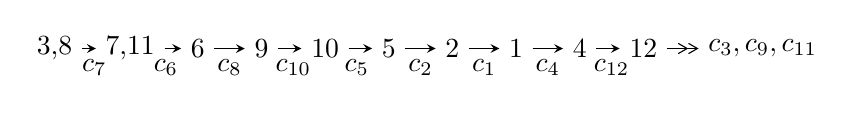
\begin{tikzpicture}[x=23pt, y=7pt]
	% node
	\node (A0) at (-1/8, 0) {3,8};
	\node (A1) at (17/16, 0) {7,11};
	\node (A2) at (17/8, 0) {6};
	\node (A3) at (25/8, 0) {9};
	\node (A4) at (33/8, 0) {10};
	\node (A5) at (41/8, 0) {5};
	\node (A6) at (49/8, 0) {2};
	\node (A7) at (57/8, 0) {1};
	\node (A8) at (65/8, 0) {4};
	\node (A9) at (73/8, 0) {12};
	\node (C1) at (1/2, -1) {$c_{7}$};
	\node (C2) at (13/8, -1) {$c_{6}$};
	\node (C3) at (21/8, -1) {$c_{8}$};
	\node (C4) at (29/8, -1) {$c_{10}$};
	\node (C5) at (37/8, -1) {$c_{5}$};
	\node (C6) at (45/8, -1) {$c_{2}$};
	\node (C7) at (53/8, -1) {$c_{1}$};
	\node (C8) at (61/8, -1) {$c_{4}$};
	\node (C9) at (69/8, -1) {$c_{12}$};
	\node (A10) at (11, 0) {$c_{3},c_{9},c_{11}$};

	% edge
	\draw[->,>=stealth]	
	(A0) edge (A1) (A1) edge (A2) (A2) edge (A3) (A3) edge (A4) (A4) edge (A5) (A5) edge (A6) (A6) edge (A7) (A7) edge (A8) (A8) edge (A9) ;
	\draw[->>,>={angle 60}]	
	(A9) edge (A10);
\end{tikzpicture} \\ 

\end{tabular} \\

\footnotetext{
The image of knot diagram is generated by the software ``\textbf{Draw programme}" developed by Andrew Bartholomew(\url{http://www.layer8.co.uk/maths/draw/index.htm\#Running-draw}), where we modified some parts for our purpose(\url{https://github.com/CATsTAILs/LinksPainter}).
}\phantom \\ \newline 
\centering \textbf{Ideals for irreducible components\footnotemark of $X_{\text{par}}$} 
 
\begin{align*}
I^u_{1}&=\langle 
-6.07079\times10^{303} u^{80}+1.55900\times10^{304} u^{79}+\cdots+4.90378\times10^{306} b-8.03703\times10^{306},\\
\phantom{I^u_{1}}&\phantom{= \langle  }1.46094\times10^{304} u^{80}-6.01646\times10^{304} u^{79}+\cdots+4.90378\times10^{306} a-3.48928\times10^{307},\\
\phantom{I^u_{1}}&\phantom{= \langle  }u^{81}-3 u^{80}+\cdots+1024 u+1024\rangle \\
I^u_{2}&=\langle 
b,\;a^2-3 a u+5 a-21 u+34,\;u^2- u-1\rangle \\
\\
I^v_{1}&=\langle 
a,\;- v^2+b+3 v-1,\;v^4-5 v^3+7 v^2-2 v+1\rangle \\
I^v_{2}&=\langle 
a,\;-3 v^5-38 v^4-14 v^3-295 v^2+67 b-19 v-65,\;v^6+8 v^4+2 v^3+4 v^2+v+1\rangle \\
\end{align*}
\raggedright * 4 irreducible components of $\dim_{\mathbb{C}}=0$, with total 95 representations.\\
\footnotetext{All coefficients of polynomials are rational numbers. But the coefficients are sometimes approximated in decimal forms when there is not enough margin.}
\newpage
\renewcommand{\arraystretch}{1}
\centering \section*{I. $I^u_{1}= \langle -6.07\times10^{303} u^{80}+1.56\times10^{304} u^{79}+\cdots+4.90\times10^{306} b-8.04\times10^{306},\;1.46\times10^{304} u^{80}-6.02\times10^{304} u^{79}+\cdots+4.90\times10^{306} a-3.49\times10^{307},\;u^{81}-3 u^{80}+\cdots+1024 u+1024 \rangle$}
\flushleft \textbf{(i) Arc colorings}\\
\begin{tabular}{m{7pt} m{180pt} m{7pt} m{180pt} }
\flushright $a_{3}=$&$\begin{pmatrix}0\\u\end{pmatrix}$ \\
\flushright $a_{8}=$&$\begin{pmatrix}1\\0\end{pmatrix}$ \\
\flushright $a_{7}=$&$\begin{pmatrix}1\\- u^2\end{pmatrix}$ \\
\flushright $a_{11}=$&$\begin{pmatrix}-0.00297921 u^{80}+0.0122690 u^{79}+\cdots-18.5060 u+7.11548\\0.00123798 u^{80}-0.00317918 u^{79}+\cdots+8.06983 u+1.63894\end{pmatrix}$ \\
\flushright $a_{6}=$&$\begin{pmatrix}0.00291408 u^{80}-0.00699880 u^{79}+\cdots-21.8367 u+36.3426\\-0.000604359 u^{80}+0.00154234 u^{79}+\cdots-5.55867 u-0.574802\end{pmatrix}$ \\
\flushright $a_{9}=$&$\begin{pmatrix}-0.00467296 u^{80}+0.0119450 u^{79}+\cdots-39.3868 u-6.00265\\-0.00154134 u^{80}+0.00547407 u^{79}+\cdots-6.57065 u+2.38699\end{pmatrix}$ \\
\flushright $a_{10}=$&$\begin{pmatrix}-0.00421719 u^{80}+0.0154482 u^{79}+\cdots-26.5758 u+5.47653\\0.00123798 u^{80}-0.00317918 u^{79}+\cdots+8.06983 u+1.63894\end{pmatrix}$ \\
\flushright $a_{5}=$&$\begin{pmatrix}-0.00342207 u^{80}+0.0108220 u^{79}+\cdots-17.4933 u-1.23720\\0.00111382 u^{80}-0.00415508 u^{79}+\cdots+3.94295 u-2.65104\end{pmatrix}$ \\
\flushright $a_{2}=$&$\begin{pmatrix}0.00230825 u^{80}-0.00666691 u^{79}+\cdots+13.5504 u+3.88824\\0.00111382 u^{80}-0.00415508 u^{79}+\cdots+3.94295 u-2.65104\end{pmatrix}$ \\
\flushright $a_{1}=$&$\begin{pmatrix}0.00230825 u^{80}-0.00666691 u^{79}+\cdots+13.5504 u+3.88824\\0.00154134 u^{80}-0.00547407 u^{79}+\cdots+6.57065 u-2.38699\end{pmatrix}$ \\
\flushright $a_{4}=$&$\begin{pmatrix}- u\\u\end{pmatrix}$ \\
\flushright $a_{12}=$&$\begin{pmatrix}-0.00259882 u^{80}+0.0103269 u^{79}+\cdots-11.5768 u+3.13075\\0.00426527 u^{80}-0.0133743 u^{79}+\cdots+18.6658 u-0.457794\end{pmatrix}$\\&\end{tabular}
\flushleft \textbf{(ii) Obstruction class $= -1$}\\~\\
\flushleft \textbf{(iii) Cusp Shapes $= 0.0207517 u^{80}-0.0712635 u^{79}+\cdots+7.67115 u+25.2859$}\\~\\
\newpage\renewcommand{\arraystretch}{1}
\flushleft \textbf{(iv) u-Polynomials at the component}\newline \\
\begin{tabular}{m{50pt}|m{274pt}}
Crossings & \hspace{64pt}u-Polynomials at each crossing \\
\hline $$\begin{aligned}c_{1}\end{aligned}$$&$\begin{aligned}
&u^{81}+33 u^{80}+\cdots+130 u+1
\end{aligned}$\\
\hline $$\begin{aligned}c_{2},c_{4}\end{aligned}$$&$\begin{aligned}
&u^{81}-13 u^{80}+\cdots-12 u+1
\end{aligned}$\\
\hline $$\begin{aligned}c_{3},c_{7}\end{aligned}$$&$\begin{aligned}
&u^{81}-3 u^{80}+\cdots+1024 u+1024
\end{aligned}$\\
\hline $$\begin{aligned}c_{5}\end{aligned}$$&$\begin{aligned}
&u^{81}+5 u^{80}+\cdots-47488 u+22208
\end{aligned}$\\
\hline $$\begin{aligned}c_{6}\end{aligned}$$&$\begin{aligned}
&u^{81}+u^{80}+\cdots+8905262 u+2124511
\end{aligned}$\\
\hline $$\begin{aligned}c_{8}\end{aligned}$$&$\begin{aligned}
&u^{81}-4 u^{80}+\cdots-5 u+1
\end{aligned}$\\
\hline $$\begin{aligned}c_{9},c_{12}\end{aligned}$$&$\begin{aligned}
&u^{81}+4 u^{80}+\cdots+83 u-1
\end{aligned}$\\
\hline $$\begin{aligned}c_{10}\end{aligned}$$&$\begin{aligned}
&u^{81}+8 u^{80}+\cdots+256 u+16
\end{aligned}$\\
\hline $$\begin{aligned}c_{11}\end{aligned}$$&$\begin{aligned}
&u^{81}+30 u^{80}+\cdots+6303 u-1
\end{aligned}$\\
\hline
\end{tabular}\\~\\
\newpage\renewcommand{\arraystretch}{1}
\flushleft \textbf{(v) Riley Polynomials at the component}\newline \\
\begin{tabular}{m{50pt}|m{274pt}}
Crossings & \hspace{64pt}Riley Polynomials at each crossing \\
\hline $$\begin{aligned}c_{1}\end{aligned}$$&$\begin{aligned}
&y^{81}+43 y^{80}+\cdots+5274 y-1
\end{aligned}$\\
\hline $$\begin{aligned}c_{2},c_{4}\end{aligned}$$&$\begin{aligned}
&y^{81}-33 y^{80}+\cdots+130 y-1
\end{aligned}$\\
\hline $$\begin{aligned}c_{3},c_{7}\end{aligned}$$&$\begin{aligned}
&y^{81}+57 y^{80}+\cdots-27787264 y-1048576
\end{aligned}$\\
\hline $$\begin{aligned}c_{5}\end{aligned}$$&$\begin{aligned}
&y^{81}+103 y^{80}+\cdots-19451522048 y-493195264
\end{aligned}$\\
\hline $$\begin{aligned}c_{6}\end{aligned}$$&$\begin{aligned}
&y^{81}+47 y^{80}+\cdots+59668081079090 y-4513546989121
\end{aligned}$\\
\hline $$\begin{aligned}c_{8}\end{aligned}$$&$\begin{aligned}
&y^{81}-6 y^{80}+\cdots+11 y-1
\end{aligned}$\\
\hline $$\begin{aligned}c_{9},c_{12}\end{aligned}$$&$\begin{aligned}
&y^{81}+30 y^{80}+\cdots+6303 y-1
\end{aligned}$\\
\hline $$\begin{aligned}c_{10}\end{aligned}$$&$\begin{aligned}
&y^{81}-20 y^{80}+\cdots-1152 y-256
\end{aligned}$\\
\hline $$\begin{aligned}c_{11}\end{aligned}$$&$\begin{aligned}
&y^{81}+46 y^{80}+\cdots+39786411 y-1
\end{aligned}$\\
\hline
\end{tabular}\\~\\
\newpage\flushleft \textbf{(vi) Complex Volumes and Cusp Shapes}
$$\begin{array}{c|c|c}  
\text{Solutions to }I^u_{1}& \I (\text{vol} + \sqrt{-1}CS) & \text{Cusp shape}\\
 \hline 
\begin{aligned}
u &= \phantom{-}0.890661 + 0.321140 I \\
a &= \phantom{-}0.442794 - 0.506116 I \\
b &= -1.003170 - 0.678335 I\end{aligned}
 & -3.72961 + 3.73093 I & \phantom{-0.000000 } 0 \\ \hline\begin{aligned}
u &= \phantom{-}0.890661 - 0.321140 I \\
a &= \phantom{-}0.442794 + 0.506116 I \\
b &= -1.003170 + 0.678335 I\end{aligned}
 & -3.72961 - 3.73093 I & \phantom{-0.000000 } 0 \\ \hline\begin{aligned}
u &= -0.880183 + 0.328930 I \\
a &= -0.192285 + 0.385420 I \\
b &= -0.519092 + 0.581351 I\end{aligned}
 & -2.15630 + 0.07606 I & \phantom{-0.000000 } 0 \\ \hline\begin{aligned}
u &= -0.880183 - 0.328930 I \\
a &= -0.192285 - 0.385420 I \\
b &= -0.519092 - 0.581351 I\end{aligned}
 & -2.15630 - 0.07606 I & \phantom{-0.000000 } 0 \\ \hline\begin{aligned}
u &= \phantom{-}0.336499 + 0.810387 I \\
a &= -2.50423 + 0.47126 I \\
b &= -0.722560 + 0.702901 I\end{aligned}
 & -4.60609 - 1.52975 I & -9.48461 + 4.54719 I \\ \hline\begin{aligned}
u &= \phantom{-}0.336499 - 0.810387 I \\
a &= -2.50423 - 0.47126 I \\
b &= -0.722560 - 0.702901 I\end{aligned}
 & -4.60609 + 1.52975 I & -9.48461 - 4.54719 I \\ \hline\begin{aligned}
u &= -0.086690 + 1.153850 I \\
a &= \phantom{-}1.217480 + 0.665727 I \\
b &= \phantom{-}0.759691 - 0.320662 I\end{aligned}
 & \phantom{-}1.73887 + 0.56914 I & \phantom{-0.000000 } 0 \\ \hline\begin{aligned}
u &= -0.086690 - 1.153850 I \\
a &= \phantom{-}1.217480 - 0.665727 I \\
b &= \phantom{-}0.759691 + 0.320662 I\end{aligned}
 & \phantom{-}1.73887 - 0.56914 I & \phantom{-0.000000 } 0 \\ \hline\begin{aligned}
u &= -0.439042 + 1.154740 I \\
a &= \phantom{-}0.732667 - 0.568454 I \\
b &= \phantom{-}0.668186 + 0.622788 I\end{aligned}
 & \phantom{-}0.95414 + 4.42889 I & \phantom{-0.000000 } 0 \\ \hline\begin{aligned}
u &= -0.439042 - 1.154740 I \\
a &= \phantom{-}0.732667 + 0.568454 I \\
b &= \phantom{-}0.668186 - 0.622788 I\end{aligned}
 & \phantom{-}0.95414 - 4.42889 I & \phantom{-0.000000 } 0\\
 \hline 
 \end{array}$$\newpage$$\begin{array}{c|c|c}  
\text{Solutions to }I^u_{1}& \I (\text{vol} + \sqrt{-1}CS) & \text{Cusp shape}\\
 \hline 
\begin{aligned}
u &= \phantom{-}0.757611 + 0.003546 I \\
a &= -0.24323 - 2.40067 I \\
b &= -0.675714 + 1.029340 I\end{aligned}
 & -0.12016 + 3.83503 I & -2.19897 - 9.50011 I \\ \hline\begin{aligned}
u &= \phantom{-}0.757611 - 0.003546 I \\
a &= -0.24323 + 2.40067 I \\
b &= -0.675714 - 1.029340 I\end{aligned}
 & -0.12016 - 3.83503 I & -2.19897 + 9.50011 I \\ \hline\begin{aligned}
u &= -0.123794 + 1.279290 I \\
a &= -1.50264 - 0.27690 I \\
b &= -1.68690 - 0.59992 I\end{aligned}
 & \phantom{-}0.90648 + 3.26112 I & \phantom{-0.000000 } 0 \\ \hline\begin{aligned}
u &= -0.123794 - 1.279290 I \\
a &= -1.50264 + 0.27690 I \\
b &= -1.68690 + 0.59992 I\end{aligned}
 & \phantom{-}0.90648 - 3.26112 I & \phantom{-0.000000 } 0 \\ \hline\begin{aligned}
u &= -0.239752 + 1.287670 I \\
a &= \phantom{-}0.863701 - 0.766311 I \\
b &= \phantom{-}0.941346 - 0.469197 I\end{aligned}
 & \phantom{-}0.58736 - 1.68614 I & \phantom{-0.000000 } 0 \\ \hline\begin{aligned}
u &= -0.239752 - 1.287670 I \\
a &= \phantom{-}0.863701 + 0.766311 I \\
b &= \phantom{-}0.941346 + 0.469197 I\end{aligned}
 & \phantom{-}0.58736 + 1.68614 I & \phantom{-0.000000 } 0 \\ \hline\begin{aligned}
u &= \phantom{-}1.357180 + 0.050552 I \\
a &= \phantom{-}0.0152362 - 0.1308150 I \\
b &= \phantom{-}1.112340 + 0.692920 I\end{aligned}
 & \phantom{-}2.74432 + 4.49163 I & \phantom{-0.000000 } 0 \\ \hline\begin{aligned}
u &= \phantom{-}1.357180 - 0.050552 I \\
a &= \phantom{-}0.0152362 + 0.1308150 I \\
b &= \phantom{-}1.112340 - 0.692920 I\end{aligned}
 & \phantom{-}2.74432 - 4.49163 I & \phantom{-0.000000 } 0 \\ \hline\begin{aligned}
u &= \phantom{-}0.616988 + 0.161976 I \\
a &= -0.42521 + 1.42820 I \\
b &= \phantom{-}0.910146 - 0.634484 I\end{aligned}
 & \phantom{-}1.29375 - 1.45245 I & \phantom{-}3.62930 + 4.86424 I \\ \hline\begin{aligned}
u &= \phantom{-}0.616988 - 0.161976 I \\
a &= -0.42521 - 1.42820 I \\
b &= \phantom{-}0.910146 + 0.634484 I\end{aligned}
 & \phantom{-}1.29375 + 1.45245 I & \phantom{-}3.62930 - 4.86424 I\\
 \hline 
 \end{array}$$\newpage$$\begin{array}{c|c|c}  
\text{Solutions to }I^u_{1}& \I (\text{vol} + \sqrt{-1}CS) & \text{Cusp shape}\\
 \hline 
\begin{aligned}
u &= \phantom{-}0.077263 + 0.631820 I \\
a &= \phantom{-}0.116121 - 0.173911 I \\
b &= -0.297655 - 1.305260 I\end{aligned}
 & -5.47007 - 0.37522 I & -3.64589 + 3.20724 I \\ \hline\begin{aligned}
u &= \phantom{-}0.077263 - 0.631820 I \\
a &= \phantom{-}0.116121 + 0.173911 I \\
b &= -0.297655 + 1.305260 I\end{aligned}
 & -5.47007 + 0.37522 I & -3.64589 - 3.20724 I \\ \hline\begin{aligned}
u &= -0.455347 + 0.441128 I \\
a &= -1.71279 - 1.55684 I \\
b &= \phantom{-}0.569120 - 0.233874 I\end{aligned}
 & -1.004280 - 0.810007 I & -4.84130 - 2.46574 I \\ \hline\begin{aligned}
u &= -0.455347 - 0.441128 I \\
a &= -1.71279 + 1.55684 I \\
b &= \phantom{-}0.569120 + 0.233874 I\end{aligned}
 & -1.004280 + 0.810007 I & -4.84130 + 2.46574 I \\ \hline\begin{aligned}
u &= -0.020461 + 0.617454 I \\
a &= -0.073029 - 0.151006 I \\
b &= \phantom{-}0.391395 + 1.125760 I\end{aligned}
 & -1.20619 + 3.00339 I & \phantom{-}2.21341 - 3.98452 I \\ \hline\begin{aligned}
u &= -0.020461 - 0.617454 I \\
a &= -0.073029 + 0.151006 I \\
b &= \phantom{-}0.391395 - 1.125760 I\end{aligned}
 & -1.20619 - 3.00339 I & \phantom{-}2.21341 + 3.98452 I \\ \hline\begin{aligned}
u &= -0.612334\phantom{ +0.000000I} \\
a &= -0.700707\phantom{ +0.000000I} \\
b &= -0.112219\phantom{ +0.000000I}\end{aligned}
 & -1.00318\phantom{ +0.000000I} & -10.1710\phantom{ +0.000000I} \\ \hline\begin{aligned}
u &= -0.154661 + 1.382630 I \\
a &= -0.18086 - 1.44008 I \\
b &= -0.018338 + 0.694246 I\end{aligned}
 & \phantom{-}3.68961 + 0.58365 I & \phantom{-0.000000 } 0 \\ \hline\begin{aligned}
u &= -0.154661 - 1.382630 I \\
a &= -0.18086 + 1.44008 I \\
b &= -0.018338 - 0.694246 I\end{aligned}
 & \phantom{-}3.68961 - 0.58365 I & \phantom{-0.000000 } 0 \\ \hline\begin{aligned}
u &= -0.603292 + 0.010555 I \\
a &= -1.93148 - 11.47890 I \\
b &= -0.015568 + 0.155944 I\end{aligned}
 & -1.02453 - 2.05291 I & -171.972 + 28.532 I\\
 \hline 
 \end{array}$$\newpage$$\begin{array}{c|c|c}  
\text{Solutions to }I^u_{1}& \I (\text{vol} + \sqrt{-1}CS) & \text{Cusp shape}\\
 \hline 
\begin{aligned}
u &= -0.603292 - 0.010555 I \\
a &= -1.93148 + 11.47890 I \\
b &= -0.015568 - 0.155944 I\end{aligned}
 & -1.02453 + 2.05291 I & -171.972 - 28.532 I \\ \hline\begin{aligned}
u &= -0.277078 + 1.371800 I \\
a &= \phantom{-}0.68222 + 1.38332 I \\
b &= \phantom{-}0.260117 - 0.634813 I\end{aligned}
 & \phantom{-}3.45045 + 5.35632 I & \phantom{-0.000000 } 0 \\ \hline\begin{aligned}
u &= -0.277078 - 1.371800 I \\
a &= \phantom{-}0.68222 - 1.38332 I \\
b &= \phantom{-}0.260117 + 0.634813 I\end{aligned}
 & \phantom{-}3.45045 - 5.35632 I & \phantom{-0.000000 } 0 \\ \hline\begin{aligned}
u &= \phantom{-}0.50450 + 1.33076 I \\
a &= -1.49367 - 0.17378 I \\
b &= -1.60038 + 1.10707 I\end{aligned}
 & -0.35544 - 9.04141 I & \phantom{-0.000000 } 0 \\ \hline\begin{aligned}
u &= \phantom{-}0.50450 - 1.33076 I \\
a &= -1.49367 + 0.17378 I \\
b &= -1.60038 - 1.10707 I\end{aligned}
 & -0.35544 + 9.04141 I & \phantom{-0.000000 } 0 \\ \hline\begin{aligned}
u &= -0.00539 + 1.42943 I \\
a &= -1.054200 + 0.533535 I \\
b &= -0.975011 + 0.566121 I\end{aligned}
 & -0.36837 - 7.06216 I & \phantom{-0.000000 } 0 \\ \hline\begin{aligned}
u &= -0.00539 - 1.42943 I \\
a &= -1.054200 - 0.533535 I \\
b &= -0.975011 - 0.566121 I\end{aligned}
 & -0.36837 + 7.06216 I & \phantom{-0.000000 } 0 \\ \hline\begin{aligned}
u &= \phantom{-}0.05609 + 1.43328 I \\
a &= -0.951617 + 0.465595 I \\
b &= -0.99821 + 1.90356 I\end{aligned}
 & \phantom{-}5.23560 + 2.02485 I & \phantom{-0.000000 } 0 \\ \hline\begin{aligned}
u &= \phantom{-}0.05609 - 1.43328 I \\
a &= -0.951617 - 0.465595 I \\
b &= -0.99821 - 1.90356 I\end{aligned}
 & \phantom{-}5.23560 - 2.02485 I & \phantom{-0.000000 } 0 \\ \hline\begin{aligned}
u &= -0.060321 + 0.542689 I \\
a &= -0.1220830 + 0.0599037 I \\
b &= -0.495796 - 1.199200 I\end{aligned}
 & -3.86039 + 7.78753 I & \phantom{-}2.42285 - 9.44743 I\\
 \hline 
 \end{array}$$\newpage$$\begin{array}{c|c|c}  
\text{Solutions to }I^u_{1}& \I (\text{vol} + \sqrt{-1}CS) & \text{Cusp shape}\\
 \hline 
\begin{aligned}
u &= -0.060321 - 0.542689 I \\
a &= -0.1220830 - 0.0599037 I \\
b &= -0.495796 + 1.199200 I\end{aligned}
 & -3.86039 - 7.78753 I & \phantom{-}2.42285 + 9.44743 I \\ \hline\begin{aligned}
u &= -0.21037 + 1.44375 I \\
a &= -1.271590 + 0.097495 I \\
b &= -0.747773 - 0.139398 I\end{aligned}
 & \phantom{-}4.09035 + 3.09672 I & \phantom{-0.000000 } 0 \\ \hline\begin{aligned}
u &= -0.21037 - 1.44375 I \\
a &= -1.271590 - 0.097495 I \\
b &= -0.747773 + 0.139398 I\end{aligned}
 & \phantom{-}4.09035 - 3.09672 I & \phantom{-0.000000 } 0 \\ \hline\begin{aligned}
u &= \phantom{-}0.35709 + 1.43000 I \\
a &= -0.667194 - 0.762996 I \\
b &= -1.46916 - 1.65478 I\end{aligned}
 & \phantom{-}4.66300 - 8.19652 I & \phantom{-0.000000 } 0 \\ \hline\begin{aligned}
u &= \phantom{-}0.35709 - 1.43000 I \\
a &= -0.667194 + 0.762996 I \\
b &= -1.46916 + 1.65478 I\end{aligned}
 & \phantom{-}4.66300 + 8.19652 I & \phantom{-0.000000 } 0 \\ \hline\begin{aligned}
u &= \phantom{-}1.45915 + 0.22710 I \\
a &= -0.1005500 + 0.0324263 I \\
b &= -1.114300 - 0.737613 I\end{aligned}
 & \phantom{-}1.48186 + 10.21890 I & \phantom{-0.000000 } 0 \\ \hline\begin{aligned}
u &= \phantom{-}1.45915 - 0.22710 I \\
a &= -0.1005500 - 0.0324263 I \\
b &= -1.114300 + 0.737613 I\end{aligned}
 & \phantom{-}1.48186 - 10.21890 I & \phantom{-0.000000 } 0 \\ \hline\begin{aligned}
u &= -0.458462 + 0.233945 I \\
a &= \phantom{-}1.32051 - 7.34173 I \\
b &= \phantom{-}0.190371 + 0.428906 I\end{aligned}
 & -1.11518 + 1.63608 I & -22.5154 - 16.4209 I \\ \hline\begin{aligned}
u &= -0.458462 - 0.233945 I \\
a &= \phantom{-}1.32051 + 7.34173 I \\
b &= \phantom{-}0.190371 - 0.428906 I\end{aligned}
 & -1.11518 - 1.63608 I & -22.5154 + 16.4209 I \\ \hline\begin{aligned}
u &= -1.42270 + 0.44570 I \\
a &= \phantom{-}0.0501638 - 0.1205880 I \\
b &= \phantom{-}0.955191 + 0.178009 I\end{aligned}
 & \phantom{-}1.96531 - 1.49483 I & \phantom{-0.000000 } 0\\
 \hline 
 \end{array}$$\newpage$$\begin{array}{c|c|c}  
\text{Solutions to }I^u_{1}& \I (\text{vol} + \sqrt{-1}CS) & \text{Cusp shape}\\
 \hline 
\begin{aligned}
u &= -1.42270 - 0.44570 I \\
a &= \phantom{-}0.0501638 + 0.1205880 I \\
b &= \phantom{-}0.955191 - 0.178009 I\end{aligned}
 & \phantom{-}1.96531 + 1.49483 I & \phantom{-0.000000 } 0 \\ \hline\begin{aligned}
u &= \phantom{-}0.16545 + 1.48707 I \\
a &= \phantom{-}1.079910 + 0.634140 I \\
b &= \phantom{-}1.82794 + 1.28596 I\end{aligned}
 & \phantom{-}7.13557 - 1.25582 I & \phantom{-0.000000 } 0 \\ \hline\begin{aligned}
u &= \phantom{-}0.16545 - 1.48707 I \\
a &= \phantom{-}1.079910 - 0.634140 I \\
b &= \phantom{-}1.82794 - 1.28596 I\end{aligned}
 & \phantom{-}7.13557 + 1.25582 I & \phantom{-0.000000 } 0 \\ \hline\begin{aligned}
u &= \phantom{-}0.25605 + 1.48232 I \\
a &= \phantom{-}1.292240 - 0.234967 I \\
b &= \phantom{-}1.47994 - 1.70675 I\end{aligned}
 & \phantom{-}6.96738 - 5.09561 I & \phantom{-0.000000 } 0 \\ \hline\begin{aligned}
u &= \phantom{-}0.25605 - 1.48232 I \\
a &= \phantom{-}1.292240 + 0.234967 I \\
b &= \phantom{-}1.47994 + 1.70675 I\end{aligned}
 & \phantom{-}6.96738 + 5.09561 I & \phantom{-0.000000 } 0 \\ \hline\begin{aligned}
u &= \phantom{-}0.412488 + 0.213180 I \\
a &= -0.80784 - 1.70565 I \\
b &= \phantom{-}0.531910 + 0.798490 I\end{aligned}
 & \phantom{-}1.15026 + 1.50439 I & \phantom{-}2.46877 - 2.61626 I \\ \hline\begin{aligned}
u &= \phantom{-}0.412488 - 0.213180 I \\
a &= -0.80784 + 1.70565 I \\
b &= \phantom{-}0.531910 - 0.798490 I\end{aligned}
 & \phantom{-}1.15026 - 1.50439 I & \phantom{-}2.46877 + 2.61626 I \\ \hline\begin{aligned}
u &= -1.54169 + 0.19466 I \\
a &= -0.1029750 + 0.0228323 I \\
b &= -0.958935 - 0.306788 I\end{aligned}
 & \phantom{-}1.52644 + 3.83350 I & \phantom{-0.000000 } 0 \\ \hline\begin{aligned}
u &= -1.54169 - 0.19466 I \\
a &= -0.1029750 - 0.0228323 I \\
b &= -0.958935 + 0.306788 I\end{aligned}
 & \phantom{-}1.52644 - 3.83350 I & \phantom{-0.000000 } 0 \\ \hline\begin{aligned}
u &= -0.110600 + 0.423339 I \\
a &= -8.26925 + 1.55023 I \\
b &= -0.443406 - 0.498696 I\end{aligned}
 & -1.63060 - 2.73282 I & \phantom{-}5.99931 - 8.61315 I\\
 \hline 
 \end{array}$$\newpage$$\begin{array}{c|c|c}  
\text{Solutions to }I^u_{1}& \I (\text{vol} + \sqrt{-1}CS) & \text{Cusp shape}\\
 \hline 
\begin{aligned}
u &= -0.110600 - 0.423339 I \\
a &= -8.26925 - 1.55023 I \\
b &= -0.443406 + 0.498696 I\end{aligned}
 & -1.63060 + 2.73282 I & \phantom{-}5.99931 + 8.61315 I \\ \hline\begin{aligned}
u &= \phantom{-}1.59287 + 0.05128 I \\
a &= -0.0398353 - 0.0628798 I \\
b &= -0.149905 - 0.238308 I\end{aligned}
 & -8.92096 - 1.95711 I & \phantom{-0.000000 } 0 \\ \hline\begin{aligned}
u &= \phantom{-}1.59287 - 0.05128 I \\
a &= -0.0398353 + 0.0628798 I \\
b &= -0.149905 + 0.238308 I\end{aligned}
 & -8.92096 + 1.95711 I & \phantom{-0.000000 } 0 \\ \hline\begin{aligned}
u &= \phantom{-}0.66734 + 1.50573 I \\
a &= \phantom{-}1.297240 + 0.255032 I \\
b &= \phantom{-}1.33285 - 1.17939 I\end{aligned}
 & \phantom{-}7.29123 - 11.70270 I & \phantom{-0.000000 } 0 \\ \hline\begin{aligned}
u &= \phantom{-}0.66734 - 1.50573 I \\
a &= \phantom{-}1.297240 - 0.255032 I \\
b &= \phantom{-}1.33285 + 1.17939 I\end{aligned}
 & \phantom{-}7.29123 + 11.70270 I & \phantom{-0.000000 } 0 \\ \hline\begin{aligned}
u &= -0.029747 + 0.351694 I \\
a &= -2.43391 - 1.81274 I \\
b &= -0.792812 + 0.170600 I\end{aligned}
 & -0.39491 + 2.82152 I & \phantom{-}0.62625 - 4.26826 I \\ \hline\begin{aligned}
u &= -0.029747 - 0.351694 I \\
a &= -2.43391 + 1.81274 I \\
b &= -0.792812 - 0.170600 I\end{aligned}
 & -0.39491 - 2.82152 I & \phantom{-}0.62625 + 4.26826 I \\ \hline\begin{aligned}
u &= \phantom{-}0.75699 + 1.47497 I \\
a &= -1.302640 - 0.324763 I \\
b &= -1.28571 + 1.12380 I\end{aligned}
 & \phantom{-}5.4200 - 17.9748 I & \phantom{-0.000000 } 0 \\ \hline\begin{aligned}
u &= \phantom{-}0.75699 - 1.47497 I \\
a &= -1.302640 + 0.324763 I \\
b &= -1.28571 - 1.12380 I\end{aligned}
 & \phantom{-}5.4200 + 17.9748 I & \phantom{-0.000000 } 0 \\ \hline\begin{aligned}
u &= -0.36850 + 1.64315 I \\
a &= \phantom{-}1.187110 + 0.042447 I \\
b &= \phantom{-}1.42144 + 0.91410 I\end{aligned}
 & \phantom{-}9.10043 + 4.86820 I & \phantom{-0.000000 } 0\\
 \hline 
 \end{array}$$\newpage$$\begin{array}{c|c|c}  
\text{Solutions to }I^u_{1}& \I (\text{vol} + \sqrt{-1}CS) & \text{Cusp shape}\\
 \hline 
\begin{aligned}
u &= -0.36850 - 1.64315 I \\
a &= \phantom{-}1.187110 - 0.042447 I \\
b &= \phantom{-}1.42144 - 0.91410 I\end{aligned}
 & \phantom{-}9.10043 - 4.86820 I & \phantom{-0.000000 } 0 \\ \hline\begin{aligned}
u &= -0.83647 + 1.48482 I \\
a &= \phantom{-}0.742052 - 0.280001 I \\
b &= \phantom{-}0.993630 + 0.569689 I\end{aligned}
 & \phantom{-}5.25967 + 9.70670 I & \phantom{-0.000000 } 0 \\ \hline\begin{aligned}
u &= -0.83647 - 1.48482 I \\
a &= \phantom{-}0.742052 + 0.280001 I \\
b &= \phantom{-}0.993630 - 0.569689 I\end{aligned}
 & \phantom{-}5.25967 - 9.70670 I & \phantom{-0.000000 } 0 \\ \hline\begin{aligned}
u &= -0.51625 + 1.63587 I \\
a &= -1.196860 + 0.057613 I \\
b &= -1.34804 - 0.90499 I\end{aligned}
 & \phantom{-}7.63873 + 11.12540 I & \phantom{-0.000000 } 0 \\ \hline\begin{aligned}
u &= -0.51625 - 1.63587 I \\
a &= -1.196860 - 0.057613 I \\
b &= -1.34804 + 0.90499 I\end{aligned}
 & \phantom{-}7.63873 - 11.12540 I & \phantom{-0.000000 } 0 \\ \hline\begin{aligned}
u &= -0.67879 + 1.59644 I \\
a &= -0.797876 + 0.245149 I \\
b &= -0.988493 - 0.473850 I\end{aligned}
 & \phantom{-}6.21314 + 4.26930 I & \phantom{-0.000000 } 0 \\ \hline\begin{aligned}
u &= -0.67879 - 1.59644 I \\
a &= -0.797876 - 0.245149 I \\
b &= -0.988493 + 0.473850 I\end{aligned}
 & \phantom{-}6.21314 - 4.26930 I & \phantom{-0.000000 } 0 \\ \hline\begin{aligned}
u &= \phantom{-}0.63390 + 1.61836 I \\
a &= \phantom{-}0.704523 + 0.328418 I \\
b &= \phantom{-}1.173510 - 0.194303 I\end{aligned}
 & \phantom{-}7.80552 - 2.77364 I & \phantom{-0.000000 } 0 \\ \hline\begin{aligned}
u &= \phantom{-}0.63390 - 1.61836 I \\
a &= \phantom{-}0.704523 - 0.328418 I \\
b &= \phantom{-}1.173510 + 0.194303 I\end{aligned}
 & \phantom{-}7.80552 + 2.77364 I & \phantom{-0.000000 } 0 \\ \hline\begin{aligned}
u &= \phantom{-}0.42765 + 1.74880 I \\
a &= -0.765788 - 0.255230 I \\
b &= -1.156090 + 0.105237 I\end{aligned}
 & \phantom{-}8.06491 + 2.92024 I & \phantom{-0.000000 } 0\\
 \hline 
 \end{array}$$\newpage$$\begin{array}{c|c|c}  
\text{Solutions to }I^u_{1}& \I (\text{vol} + \sqrt{-1}CS) & \text{Cusp shape}\\
 \hline 
\begin{aligned}
u &= \phantom{-}0.42765 - 1.74880 I \\
a &= -0.765788 + 0.255230 I \\
b &= -1.156090 - 0.105237 I\end{aligned}
 & \phantom{-}8.06491 - 2.92024 I & \phantom{-0.000000 } 0\\
 \hline 
 \end{array}$$\newpage\newpage\renewcommand{\arraystretch}{1}
\centering \section*{II. $I^u_{2}= \langle b,\;a^2-3 a u+5 a-21 u+34,\;u^2- u-1 \rangle$}
\flushleft \textbf{(i) Arc colorings}\\
\begin{tabular}{m{7pt} m{180pt} m{7pt} m{180pt} }
\flushright $a_{3}=$&$\begin{pmatrix}0\\u\end{pmatrix}$ \\
\flushright $a_{8}=$&$\begin{pmatrix}1\\0\end{pmatrix}$ \\
\flushright $a_{7}=$&$\begin{pmatrix}1\\- u-1\end{pmatrix}$ \\
\flushright $a_{11}=$&$\begin{pmatrix}a\\0\end{pmatrix}$ \\
\flushright $a_{6}=$&$\begin{pmatrix}a u-2 a+8 u-12\\- u-1\end{pmatrix}$ \\
\flushright $a_{9}=$&$\begin{pmatrix}a-4 u+5\\3 u+2\end{pmatrix}$ \\
\flushright $a_{10}=$&$\begin{pmatrix}a\\0\end{pmatrix}$ \\
\flushright $a_{5}=$&$\begin{pmatrix}1\\- u-1\end{pmatrix}$ \\
\flushright $a_{2}=$&$\begin{pmatrix}u\\- u-1\end{pmatrix}$ \\
\flushright $a_{1}=$&$\begin{pmatrix}u\\-3 u-2\end{pmatrix}$ \\
\flushright $a_{4}=$&$\begin{pmatrix}- u\\u\end{pmatrix}$ \\
\flushright $a_{12}=$&$\begin{pmatrix}-5 a u-2 a\\21 a u+13 a\end{pmatrix}$\\&\end{tabular}
\flushleft \textbf{(ii) Obstruction class $= 1$}\\~\\
\flushleft \textbf{(iii) Cusp Shapes $= -159 a u-92 a-21 u+24$}\\~\\
\newpage\renewcommand{\arraystretch}{1}
\flushleft \textbf{(iv) u-Polynomials at the component}\newline \\
\begin{tabular}{m{50pt}|m{274pt}}
Crossings & \hspace{64pt}u-Polynomials at each crossing \\
\hline $$\begin{aligned}c_{1}\end{aligned}$$&$\begin{aligned}
&(u^2-3 u+1)^2
\end{aligned}$\\
\hline $$\begin{aligned}c_{2},c_{3}\end{aligned}$$&$\begin{aligned}
&(u^2+u-1)^2
\end{aligned}$\\
\hline $$\begin{aligned}c_{4},c_{7}\end{aligned}$$&$\begin{aligned}
&(u^2- u-1)^2
\end{aligned}$\\
\hline $$\begin{aligned}c_{5},c_{6}\end{aligned}$$&$\begin{aligned}
&u^4+3 u^3+8 u^2+3 u+1
\end{aligned}$\\
\hline $$\begin{aligned}c_{8}\end{aligned}$$&$\begin{aligned}
&(u^2+3 u+1)^2
\end{aligned}$\\
\hline $$\begin{aligned}c_{9}\end{aligned}$$&$\begin{aligned}
&(u^2+u+1)^2
\end{aligned}$\\
\hline $$\begin{aligned}c_{10}\end{aligned}$$&$\begin{aligned}
&u^4
\end{aligned}$\\
\hline $$\begin{aligned}c_{11},c_{12}\end{aligned}$$&$\begin{aligned}
&(u^2- u+1)^2
\end{aligned}$\\
\hline
\end{tabular}\\~\\
\newpage\renewcommand{\arraystretch}{1}
\flushleft \textbf{(v) Riley Polynomials at the component}\newline \\
\begin{tabular}{m{50pt}|m{274pt}}
Crossings & \hspace{64pt}Riley Polynomials at each crossing \\
\hline $$\begin{aligned}c_{1},c_{8}\end{aligned}$$&$\begin{aligned}
&(y^2-7 y+1)^2
\end{aligned}$\\
\hline $$\begin{aligned}c_{2},c_{3},c_{4}\\c_{7}\end{aligned}$$&$\begin{aligned}
&(y^2-3 y+1)^2
\end{aligned}$\\
\hline $$\begin{aligned}c_{5},c_{6}\end{aligned}$$&$\begin{aligned}
&y^4+7 y^3+48 y^2+7 y+1
\end{aligned}$\\
\hline $$\begin{aligned}c_{9},c_{11},c_{12}\end{aligned}$$&$\begin{aligned}
&(y^2+y+1)^2
\end{aligned}$\\
\hline $$\begin{aligned}c_{10}\end{aligned}$$&$\begin{aligned}
&y^4
\end{aligned}$\\
\hline
\end{tabular}\\~\\
\newpage\flushleft \textbf{(vi) Complex Volumes and Cusp Shapes}
$$\begin{array}{c|c|c}  
\text{Solutions to }I^u_{2}& \I (\text{vol} + \sqrt{-1}CS) & \text{Cusp shape}\\
 \hline 
\begin{aligned}
u &= -0.618034\phantom{ +0.000000I} \\
a &= -3.42705 + 5.93583 I \\
b &= \phantom{-0.000000 } 0\end{aligned}
 & -0.98696 + 2.02988 I & \phantom{-}15.5000 + 37.2022 I \\ \hline\begin{aligned}
u &= -0.618034\phantom{ +0.000000I} \\
a &= -3.42705 - 5.93583 I \\
b &= \phantom{-0.000000 } 0\end{aligned}
 & -0.98696 - 2.02988 I & \phantom{-}15.5000 - 37.2022 I \\ \hline\begin{aligned}
u &= \phantom{-}1.61803\phantom{ +0.000000I} \\
a &= -0.072949 + 0.126351 I \\
b &= \phantom{-0.000000 } 0\end{aligned}
 & -8.88264 + 2.02988 I & \phantom{-}15.5000 - 44.1304 I \\ \hline\begin{aligned}
u &= \phantom{-}1.61803\phantom{ +0.000000I} \\
a &= -0.072949 - 0.126351 I \\
b &= \phantom{-0.000000 } 0\end{aligned}
 & -8.88264 - 2.02988 I & \phantom{-}15.5000 + 44.1304 I\\
 \hline 
 \end{array}$$\newpage\newpage\renewcommand{\arraystretch}{1}
\centering \section*{III. $I^v_{1}= \langle a,\;- v^2+b+3 v-1,\;v^4-5 v^3+7 v^2-2 v+1 \rangle$}
\flushleft \textbf{(i) Arc colorings}\\
\begin{tabular}{m{7pt} m{180pt} m{7pt} m{180pt} }
\flushright $a_{3}=$&$\begin{pmatrix}v\\0\end{pmatrix}$ \\
\flushright $a_{8}=$&$\begin{pmatrix}1\\0\end{pmatrix}$ \\
\flushright $a_{7}=$&$\begin{pmatrix}1\\0\end{pmatrix}$ \\
\flushright $a_{11}=$&$\begin{pmatrix}0\\v^2-3 v+1\end{pmatrix}$ \\
\flushright $a_{6}=$&$\begin{pmatrix}1\\- v^3+4 v^2-4 v\end{pmatrix}$ \\
\flushright $a_{9}=$&$\begin{pmatrix}- v^3+4 v^2-4 v+1\\v^3-5 v^2+7 v-2\end{pmatrix}$ \\
\flushright $a_{10}=$&$\begin{pmatrix}- v^2+3 v-1\\v^2-3 v+1\end{pmatrix}$ \\
\flushright $a_{5}=$&$\begin{pmatrix}- v^2+3 v-1\\- v^3+5 v^2-7 v+2\end{pmatrix}$ \\
\flushright $a_{2}=$&$\begin{pmatrix}v^2-2 v+1\\v^3-5 v^2+7 v-2\end{pmatrix}$ \\
\flushright $a_{1}=$&$\begin{pmatrix}v^2-3 v+1\\v^3-5 v^2+7 v-2\end{pmatrix}$ \\
\flushright $a_{4}=$&$\begin{pmatrix}v\\0\end{pmatrix}$ \\
\flushright $a_{12}=$&$\begin{pmatrix}- v+2\\v-3\end{pmatrix}$\\&\end{tabular}
\flushleft \textbf{(ii) Obstruction class $= 1$}\\~\\
\flushleft \textbf{(iii) Cusp Shapes $= 2 v^3-6 v^2+11 v-17$}\\~\\
\newpage\renewcommand{\arraystretch}{1}
\flushleft \textbf{(iv) u-Polynomials at the component}\newline \\
\begin{tabular}{m{50pt}|m{274pt}}
Crossings & \hspace{64pt}u-Polynomials at each crossing \\
\hline $$\begin{aligned}c_{1},c_{2}\end{aligned}$$&$\begin{aligned}
&(u-1)^4
\end{aligned}$\\
\hline $$\begin{aligned}c_{3},c_{7}\end{aligned}$$&$\begin{aligned}
&u^4
\end{aligned}$\\
\hline $$\begin{aligned}c_{4}\end{aligned}$$&$\begin{aligned}
&(u+1)^4
\end{aligned}$\\
\hline $$\begin{aligned}c_{5}\end{aligned}$$&$\begin{aligned}
&u^4+3 u^3+4 u^2+3 u+2
\end{aligned}$\\
\hline $$\begin{aligned}c_{6},c_{9}\end{aligned}$$&$\begin{aligned}
&u^4+u^2+u+1
\end{aligned}$\\
\hline $$\begin{aligned}c_{8}\end{aligned}$$&$\begin{aligned}
&u^4+2 u^3+3 u^2+u+1
\end{aligned}$\\
\hline $$\begin{aligned}c_{10},c_{12}\end{aligned}$$&$\begin{aligned}
&u^4+u^2- u+1
\end{aligned}$\\
\hline $$\begin{aligned}c_{11}\end{aligned}$$&$\begin{aligned}
&u^4-2 u^3+3 u^2- u+1
\end{aligned}$\\
\hline
\end{tabular}\\~\\
\newpage\renewcommand{\arraystretch}{1}
\flushleft \textbf{(v) Riley Polynomials at the component}\newline \\
\begin{tabular}{m{50pt}|m{274pt}}
Crossings & \hspace{64pt}Riley Polynomials at each crossing \\
\hline $$\begin{aligned}c_{1},c_{2},c_{4}\end{aligned}$$&$\begin{aligned}
&(y-1)^4
\end{aligned}$\\
\hline $$\begin{aligned}c_{3},c_{7}\end{aligned}$$&$\begin{aligned}
&y^4
\end{aligned}$\\
\hline $$\begin{aligned}c_{5}\end{aligned}$$&$\begin{aligned}
&y^4- y^3+2 y^2+7 y+4
\end{aligned}$\\
\hline $$\begin{aligned}c_{6},c_{9},c_{10}\\c_{12}\end{aligned}$$&$\begin{aligned}
&y^4+2 y^3+3 y^2+y+1
\end{aligned}$\\
\hline $$\begin{aligned}c_{8},c_{11}\end{aligned}$$&$\begin{aligned}
&y^4+2 y^3+7 y^2+5 y+1
\end{aligned}$\\
\hline
\end{tabular}\\~\\
\newpage\flushleft \textbf{(vi) Complex Volumes and Cusp Shapes}
$$\begin{array}{c|c|c}  
\text{Solutions to }I^v_{1}& \I (\text{vol} + \sqrt{-1}CS) & \text{Cusp shape}\\
 \hline 
\begin{aligned}
v &= \phantom{-}0.100768 + 0.400532 I \\
a &= \phantom{-0.000000 } 0 \\
b &= \phantom{-}0.547424 - 1.120870 I\end{aligned}
 & -4.26996 - 7.64338 I & -15.0849 + 3.8174 I \\ \hline\begin{aligned}
v &= \phantom{-}0.100768 - 0.400532 I \\
a &= \phantom{-0.000000 } 0 \\
b &= \phantom{-}0.547424 + 1.120870 I\end{aligned}
 & -4.26996 + 7.64338 I & -15.0849 - 3.8174 I \\ \hline\begin{aligned}
v &= \phantom{-}2.39923 + 0.32564 I \\
a &= \phantom{-0.000000 } 0 \\
b &= -0.547424 + 0.585652 I\end{aligned}
 & -0.66484 - 1.39709 I & \phantom{-}1.58487 + 5.38446 I \\ \hline\begin{aligned}
v &= \phantom{-}2.39923 - 0.32564 I \\
a &= \phantom{-0.000000 } 0 \\
b &= -0.547424 - 0.585652 I\end{aligned}
 & -0.66484 + 1.39709 I & \phantom{-}1.58487 - 5.38446 I\\
 \hline 
 \end{array}$$\newpage\newpage\renewcommand{\arraystretch}{1}
\centering \section*{IV. $I^v_{2}= \langle a,\;-3 v^5-38 v^4+\cdots+67 b-65,\;v^6+8 v^4+2 v^3+4 v^2+v+1 \rangle$}
\flushleft \textbf{(i) Arc colorings}\\
\begin{tabular}{m{7pt} m{180pt} m{7pt} m{180pt} }
\flushright $a_{3}=$&$\begin{pmatrix}v\\0\end{pmatrix}$ \\
\flushright $a_{8}=$&$\begin{pmatrix}1\\0\end{pmatrix}$ \\
\flushright $a_{7}=$&$\begin{pmatrix}1\\0\end{pmatrix}$ \\
\flushright $a_{11}=$&$\begin{pmatrix}0\\0.0447761 v^{5}+0.567164 v^{4}+\cdots+0.283582 v+0.970149\end{pmatrix}$ \\
\flushright $a_{6}=$&$\begin{pmatrix}1\\-0.373134 v^{5}-0.0597015 v^{4}+\cdots-2.02985 v-1.41791\end{pmatrix}$ \\
\flushright $a_{9}=$&$\begin{pmatrix}-0.373134 v^{5}-0.0597015 v^{4}+\cdots-2.02985 v-0.417910\\v^5+8 v^3+2 v^2+4 v+1\end{pmatrix}$ \\
\flushright $a_{10}=$&$\begin{pmatrix}-0.0447761 v^{5}-0.567164 v^{4}+\cdots-0.283582 v-0.970149\\0.0447761 v^{5}+0.567164 v^{4}+\cdots+0.283582 v+0.970149\end{pmatrix}$ \\
\flushright $a_{5}=$&$\begin{pmatrix}0.626866 v^{5}-0.0597015 v^{4}+\cdots+1.97015 v+0.582090\\- v^5-8 v^3-2 v^2-4 v-1\end{pmatrix}$ \\
\flushright $a_{2}=$&$\begin{pmatrix}-0.626866 v^{5}+0.0597015 v^{4}+\cdots-0.970149 v-0.582090\\v^5+8 v^3+2 v^2+4 v+1\end{pmatrix}$ \\
\flushright $a_{1}=$&$\begin{pmatrix}-0.626866 v^{5}+0.0597015 v^{4}+\cdots-1.97015 v-0.582090\\v^5+8 v^3+2 v^2+4 v+1\end{pmatrix}$ \\
\flushright $a_{4}=$&$\begin{pmatrix}v\\0\end{pmatrix}$ \\
\flushright $a_{12}=$&$\begin{pmatrix}-0.567164 v^{5}+0.149254 v^{4}+\cdots-0.925373 v-0.955224\\0.776119 v^{5}+0.164179 v^{4}+\cdots+1.58209 v+2.14925\end{pmatrix}$\\&\end{tabular}
\flushleft \textbf{(ii) Obstruction class $= 1$}\\~\\
\flushleft \textbf{(iii) Cusp Shapes $= -\frac{85}{67} v^5-\frac{27}{67} v^4-\frac{620}{67} v^3-\frac{363}{67} v^2+\frac{154}{67} v-\frac{859}{67}$}\\~\\
\newpage\renewcommand{\arraystretch}{1}
\flushleft \textbf{(iv) u-Polynomials at the component}\newline \\
\begin{tabular}{m{50pt}|m{274pt}}
Crossings & \hspace{64pt}u-Polynomials at each crossing \\
\hline $$\begin{aligned}c_{1},c_{2}\end{aligned}$$&$\begin{aligned}
&(u-1)^6
\end{aligned}$\\
\hline $$\begin{aligned}c_{3},c_{7}\end{aligned}$$&$\begin{aligned}
&u^6
\end{aligned}$\\
\hline $$\begin{aligned}c_{4}\end{aligned}$$&$\begin{aligned}
&(u+1)^6
\end{aligned}$\\
\hline $$\begin{aligned}c_{5}\end{aligned}$$&$\begin{aligned}
&(u^3- u^2+1)^2
\end{aligned}$\\
\hline $$\begin{aligned}c_{6},c_{9}\end{aligned}$$&$\begin{aligned}
&u^6- u^5+2 u^4-2 u^3+2 u^2-2 u+1
\end{aligned}$\\
\hline $$\begin{aligned}c_{8}\end{aligned}$$&$\begin{aligned}
&u^6+3 u^5+4 u^4+2 u^3+1
\end{aligned}$\\
\hline $$\begin{aligned}c_{10},c_{12}\end{aligned}$$&$\begin{aligned}
&u^6+u^5+2 u^4+2 u^3+2 u^2+2 u+1
\end{aligned}$\\
\hline $$\begin{aligned}c_{11}\end{aligned}$$&$\begin{aligned}
&u^6-3 u^5+4 u^4-2 u^3+1
\end{aligned}$\\
\hline
\end{tabular}\\~\\
\newpage\renewcommand{\arraystretch}{1}
\flushleft \textbf{(v) Riley Polynomials at the component}\newline \\
\begin{tabular}{m{50pt}|m{274pt}}
Crossings & \hspace{64pt}Riley Polynomials at each crossing \\
\hline $$\begin{aligned}c_{1},c_{2},c_{4}\end{aligned}$$&$\begin{aligned}
&(y-1)^6
\end{aligned}$\\
\hline $$\begin{aligned}c_{3},c_{7}\end{aligned}$$&$\begin{aligned}
&y^6
\end{aligned}$\\
\hline $$\begin{aligned}c_{5}\end{aligned}$$&$\begin{aligned}
&(y^3- y^2+2 y-1)^2
\end{aligned}$\\
\hline $$\begin{aligned}c_{6},c_{9},c_{10}\\c_{12}\end{aligned}$$&$\begin{aligned}
&y^6+3 y^5+4 y^4+2 y^3+1
\end{aligned}$\\
\hline $$\begin{aligned}c_{8},c_{11}\end{aligned}$$&$\begin{aligned}
&y^6- y^5+4 y^4-2 y^3+8 y^2+1
\end{aligned}$\\
\hline
\end{tabular}\\~\\
\newpage\flushleft \textbf{(vi) Complex Volumes and Cusp Shapes}
$$\begin{array}{c|c|c}  
\text{Solutions to }I^v_{2}& \I (\text{vol} + \sqrt{-1}CS) & \text{Cusp shape}\\
 \hline 
\begin{aligned}
v &= \phantom{-}0.175218 + 0.614017 I \\
a &= \phantom{-0.000000 } 0 \\
b &= -0.498832 + 1.001300 I\end{aligned}
 & -1.91067 - 2.82812 I & -8.91986 + 1.90022 I \\ \hline\begin{aligned}
v &= \phantom{-}0.175218 - 0.614017 I \\
a &= \phantom{-0.000000 } 0 \\
b &= -0.498832 - 1.001300 I\end{aligned}
 & -1.91067 + 2.82812 I & -8.91986 - 1.90022 I \\ \hline\begin{aligned}
v &= -0.307599 + 0.479689 I \\
a &= \phantom{-0.000000 } 0 \\
b &= \phantom{-}0.284920 - 1.115140 I\end{aligned}
 & -6.04826\phantom{ +0.000000I} & -14.4399 + 2.5036 I \\ \hline\begin{aligned}
v &= -0.307599 - 0.479689 I \\
a &= \phantom{-0.000000 } 0 \\
b &= \phantom{-}0.284920 + 1.115140 I\end{aligned}
 & -6.04826\phantom{ +0.000000I} & -14.4399 - 2.5036 I \\ \hline\begin{aligned}
v &= \phantom{-}0.13238 + 2.74513 I \\
a &= \phantom{-0.000000 } 0 \\
b &= \phantom{-}0.713912 + 0.305839 I\end{aligned}
 & -1.91067 - 2.82812 I & -14.1402 + 3.6935 I \\ \hline\begin{aligned}
v &= \phantom{-}0.13238 - 2.74513 I \\
a &= \phantom{-0.000000 } 0 \\
b &= \phantom{-}0.713912 - 0.305839 I\end{aligned}
 & -1.91067 + 2.82812 I & -14.1402 - 3.6935 I\\
 \hline 
 \end{array}$$\newpage
\newpage\renewcommand{\arraystretch}{1}
\centering \section*{ V. u-Polynomials}
\begin{tabular}{m{50pt}|m{274pt}}
Crossings & \hspace{64pt}u-Polynomials at each crossing \\
\hline $$\begin{aligned}c_{1}\end{aligned}$$&$\begin{aligned}
&((u-1)^{10})(u^2-3 u+1)^2(u^{81}+33 u^{80}+\cdots+130 u+1)
\end{aligned}$\\
\hline $$\begin{aligned}c_{2}\end{aligned}$$&$\begin{aligned}
&((u-1)^{10})(u^2+u-1)^2(u^{81}-13 u^{80}+\cdots-12 u+1)
\end{aligned}$\\
\hline $$\begin{aligned}c_{3}\end{aligned}$$&$\begin{aligned}
&u^{10}(u^2+u-1)^2(u^{81}-3 u^{80}+\cdots+1024 u+1024)
\end{aligned}$\\
\hline $$\begin{aligned}c_{4}\end{aligned}$$&$\begin{aligned}
&((u+1)^{10})(u^2- u-1)^2(u^{81}-13 u^{80}+\cdots-12 u+1)
\end{aligned}$\\
\hline $$\begin{aligned}c_{5}\end{aligned}$$&$\begin{aligned}
&(u^3- u^2+1)^2(u^4+3 u^3+4 u^2+3 u+2)(u^4+3 u^3+8 u^2+3 u+1)\\
&\cdot(u^{81}+5 u^{80}+\cdots-47488 u+22208)
\end{aligned}$\\
\hline $$\begin{aligned}c_{6}\end{aligned}$$&$\begin{aligned}
&(u^4+u^2+u+1)(u^4+3 u^3+8 u^2+3 u+1)\\
&\cdot(u^6- u^5+2 u^4-2 u^3+2 u^2-2 u+1)\\
&\cdot(u^{81}+u^{80}+\cdots+8905262 u+2124511)
\end{aligned}$\\
\hline $$\begin{aligned}c_{7}\end{aligned}$$&$\begin{aligned}
&u^{10}(u^2- u-1)^2(u^{81}-3 u^{80}+\cdots+1024 u+1024)
\end{aligned}$\\
\hline $$\begin{aligned}c_{8}\end{aligned}$$&$\begin{aligned}
&(u^2+3 u+1)^2(u^4+2 u^3+3 u^2+u+1)(u^6+3 u^5+4 u^4+2 u^3+1)\\
&\cdot(u^{81}-4 u^{80}+\cdots-5 u+1)
\end{aligned}$\\
\hline $$\begin{aligned}c_{9}\end{aligned}$$&$\begin{aligned}
&(u^2+u+1)^2(u^4+u^2+u+1)(u^6- u^5+2 u^4-2 u^3+2 u^2-2 u+1)\\
&\cdot(u^{81}+4 u^{80}+\cdots+83 u-1)
\end{aligned}$\\
\hline $$\begin{aligned}c_{10}\end{aligned}$$&$\begin{aligned}
&u^4(u^4+u^2- u+1)(u^6+u^5+2 u^4+2 u^3+2 u^2+2 u+1)\\
&\cdot(u^{81}+8 u^{80}+\cdots+256 u+16)
\end{aligned}$\\
\hline $$\begin{aligned}c_{11}\end{aligned}$$&$\begin{aligned}
&(u^2- u+1)^2(u^4-2 u^3+3 u^2- u+1)(u^6-3 u^5+4 u^4-2 u^3+1)\\
&\cdot(u^{81}+30 u^{80}+\cdots+6303 u-1)
\end{aligned}$\\
\hline $$\begin{aligned}c_{12}\end{aligned}$$&$\begin{aligned}
&(u^2- u+1)^2(u^4+u^2- u+1)(u^6+u^5+2 u^4+2 u^3+2 u^2+2 u+1)\\
&\cdot(u^{81}+4 u^{80}+\cdots+83 u-1)
\end{aligned}$\\
\hline
\end{tabular}\newpage\renewcommand{\arraystretch}{1}
\centering \section*{ VI. Riley Polynomials}
\begin{tabular}{m{50pt}|m{274pt}}
Crossings & \hspace{64pt}Riley Polynomials at each crossing \\
\hline $$\begin{aligned}c_{1}\end{aligned}$$&$\begin{aligned}
&((y-1)^{10})(y^2-7 y+1)^2(y^{81}+43 y^{80}+\cdots+5274 y-1)
\end{aligned}$\\
\hline $$\begin{aligned}c_{2},c_{4}\end{aligned}$$&$\begin{aligned}
&((y-1)^{10})(y^2-3 y+1)^2(y^{81}-33 y^{80}+\cdots+130 y-1)
\end{aligned}$\\
\hline $$\begin{aligned}c_{3},c_{7}\end{aligned}$$&$\begin{aligned}
&y^{10}(y^2-3 y+1)^2(y^{81}+57 y^{80}+\cdots-2.77873\times10^{7} y-1048576)
\end{aligned}$\\
\hline $$\begin{aligned}c_{5}\end{aligned}$$&$\begin{aligned}
&((y^3- y^2+2 y-1)^2)(y^4- y^3+2 y^2+7 y+4)(y^4+7 y^3+\cdots+7 y+1)\\
&\cdot(y^{81}+103 y^{80}+\cdots-19451522048 y-493195264)
\end{aligned}$\\
\hline $$\begin{aligned}c_{6}\end{aligned}$$&$\begin{aligned}
&(y^4+2 y^3+3 y^2+y+1)(y^4+7 y^3+48 y^2+7 y+1)\\
&\cdot(y^6+3 y^5+4 y^4+2 y^3+1)\\
&\cdot(y^{81}+47 y^{80}+\cdots+59668081079090 y-4513546989121)
\end{aligned}$\\
\hline $$\begin{aligned}c_{8}\end{aligned}$$&$\begin{aligned}
&((y^2-7 y+1)^2)(y^4+2 y^3+\cdots+5 y+1)(y^6- y^5+\cdots+8 y^2+1)\\
&\cdot(y^{81}-6 y^{80}+\cdots+11 y-1)
\end{aligned}$\\
\hline $$\begin{aligned}c_{9},c_{12}\end{aligned}$$&$\begin{aligned}
&(y^2+y+1)^2(y^4+2 y^3+3 y^2+y+1)(y^6+3 y^5+4 y^4+2 y^3+1)\\
&\cdot(y^{81}+30 y^{80}+\cdots+6303 y-1)
\end{aligned}$\\
\hline $$\begin{aligned}c_{10}\end{aligned}$$&$\begin{aligned}
&y^4(y^4+2 y^3+3 y^2+y+1)(y^6+3 y^5+4 y^4+2 y^3+1)\\
&\cdot(y^{81}-20 y^{80}+\cdots-1152 y-256)
\end{aligned}$\\
\hline $$\begin{aligned}c_{11}\end{aligned}$$&$\begin{aligned}
&((y^2+y+1)^2)(y^4+2 y^3+\cdots+5 y+1)(y^6- y^5+\cdots+8 y^2+1)\\
&\cdot(y^{81}+46 y^{80}+\cdots+39786411 y-1)
\end{aligned}$\\
\hline
\end{tabular}
\vskip 2pc
\end{document}